\subsection{Winston cones refurbishment}

\begin{figure}[hbt]
	\centering
	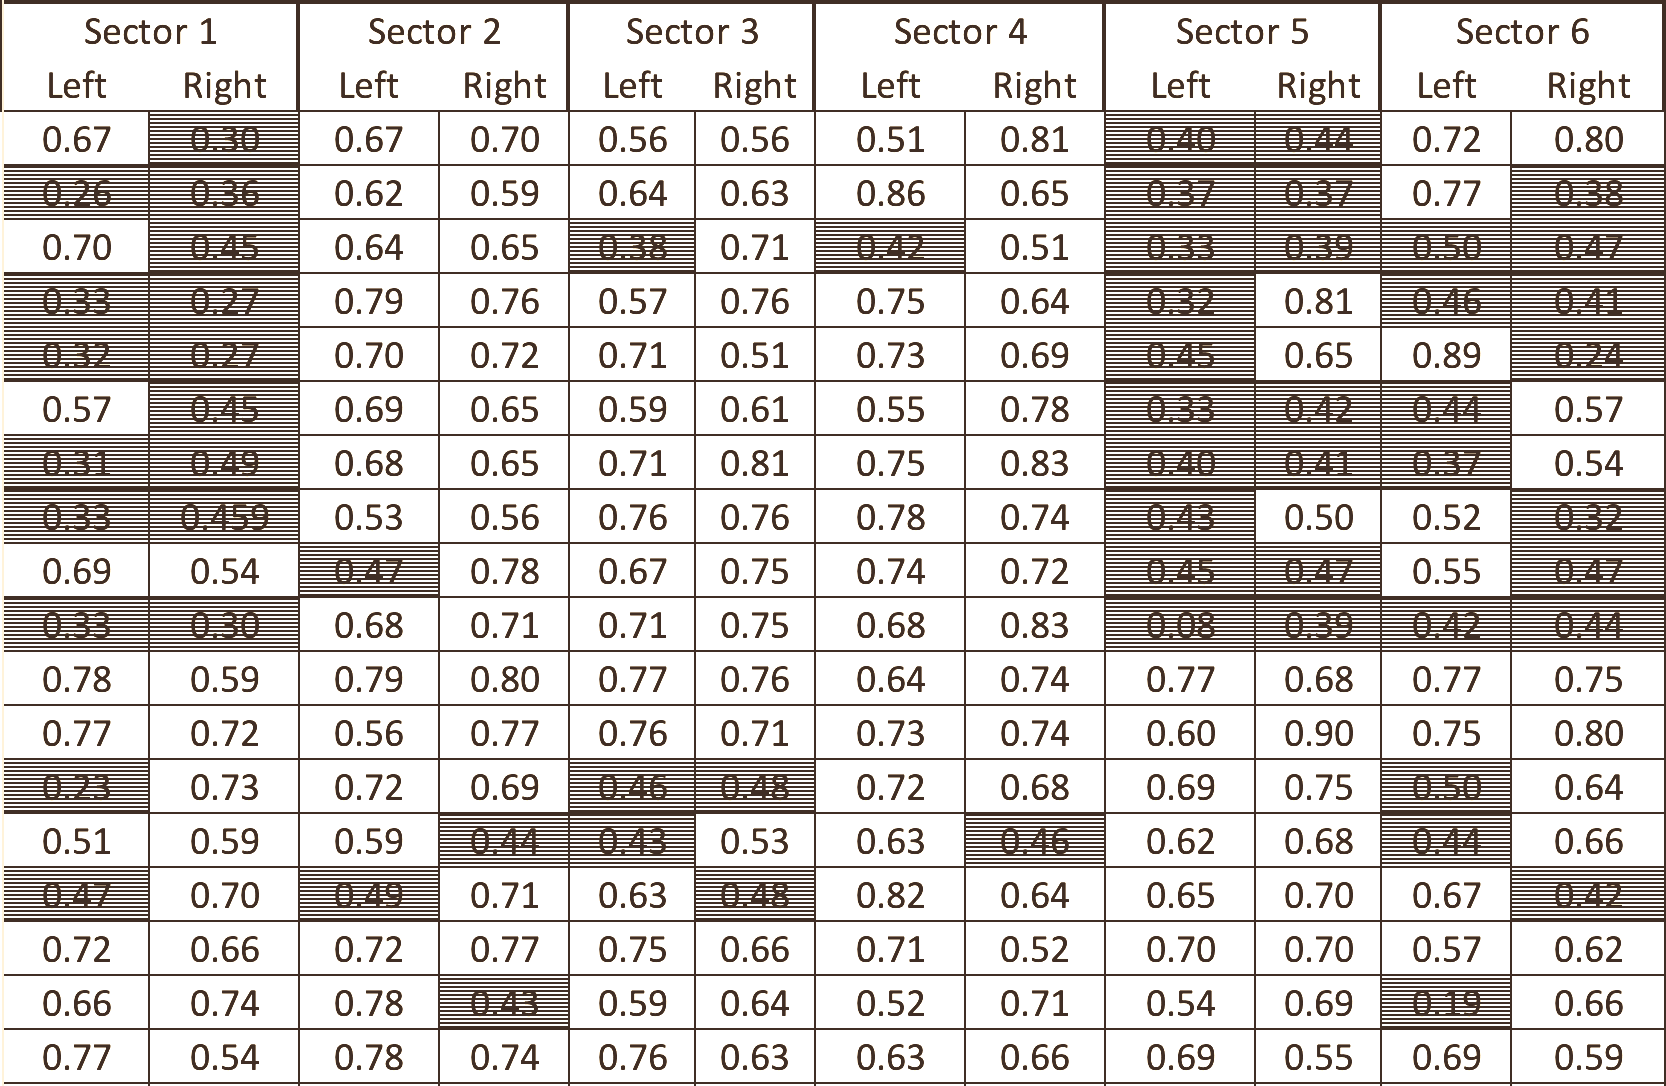
\includegraphics[width=1.0\columnwidth,keepaspectratio]{img/wcStatusBefore.png}
	\caption{Top view of the back-wall of the LTCC. A stainless steel bar encapsulate a sandwich wall of aluminum and foam. On the left and right side
			of the frame a new patch panel allow for 3 hermetical connectors (1 HV, 2 signals) from each PTM. }
	\label{fig:wcStatusBefore}
\end{figure}


\begin{figure}[hbt]
	\centering
	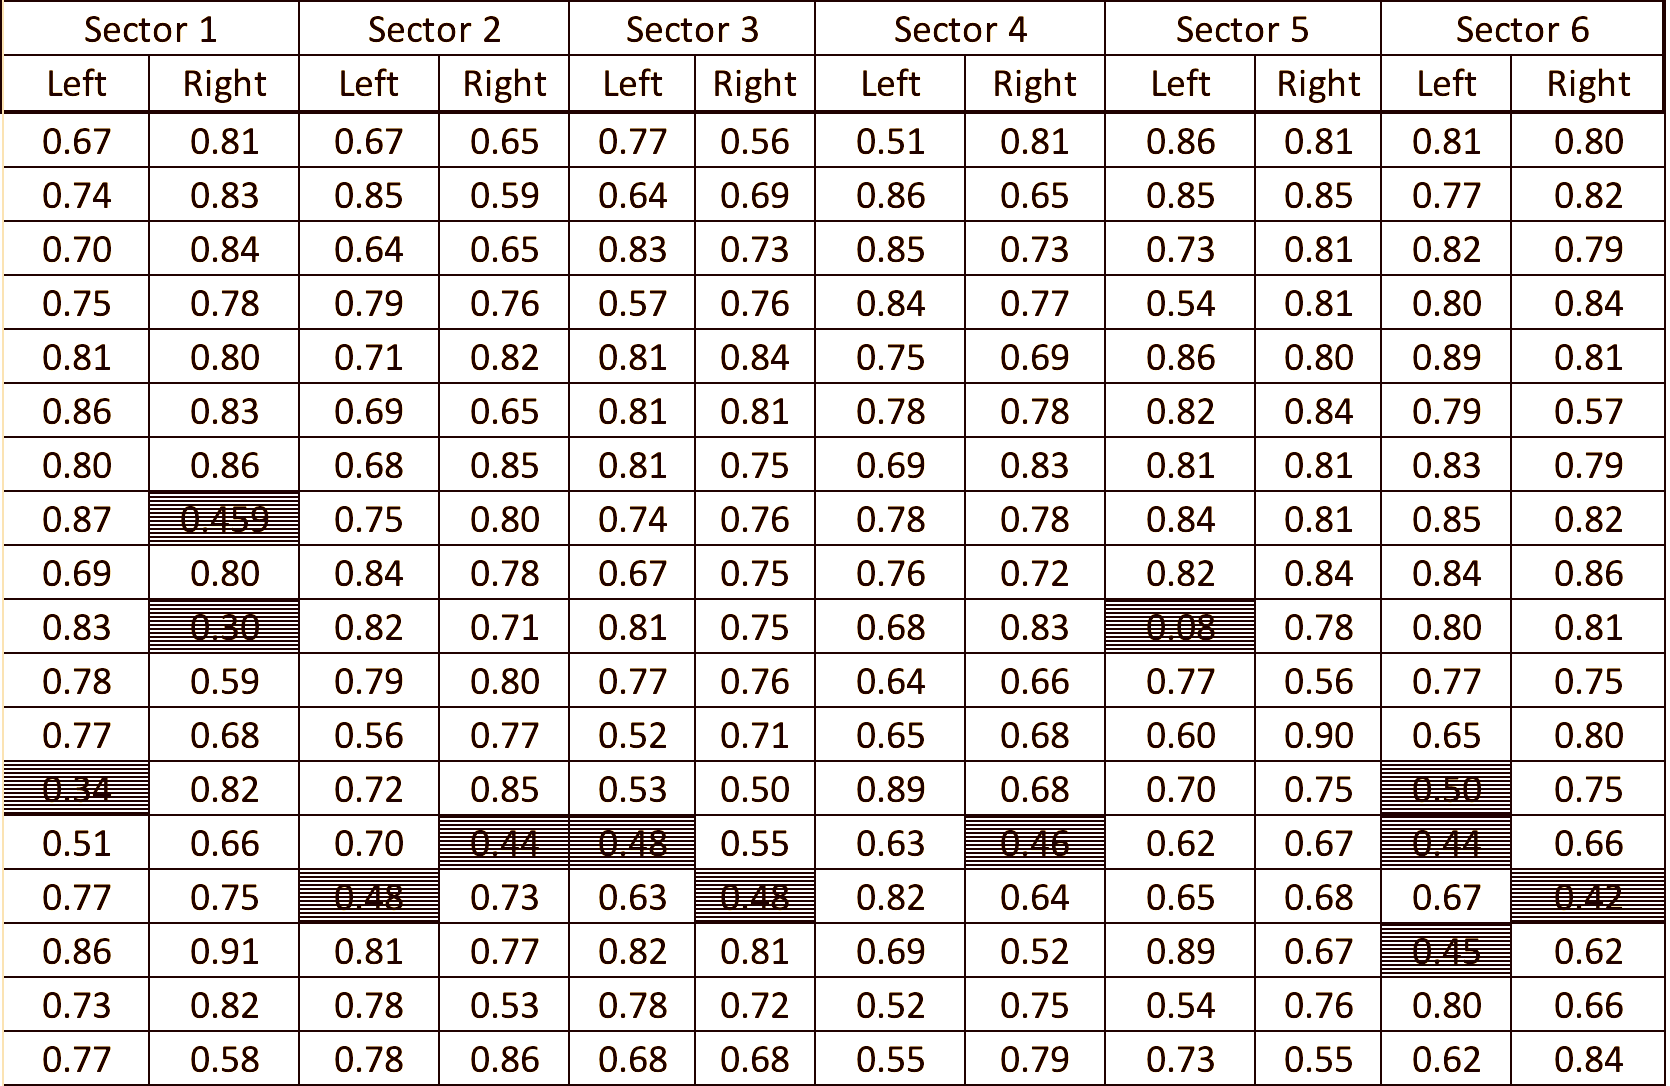
\includegraphics[width=1.0\columnwidth,keepaspectratio]{img/wcStatusAfter.png}
	\caption{Top view of the back-wall of the LTCC. A stainless steel bar encapsulate a sandwich wall of aluminum and foam. On the left and right side
			of the frame a new patch panel allow for 3 hermetical connectors (1 HV, 2 signals) from each PTM. }
	\label{fig:wcStatusAfter}
\end{figure}

\begin{figure}[hbt]
	\centering
	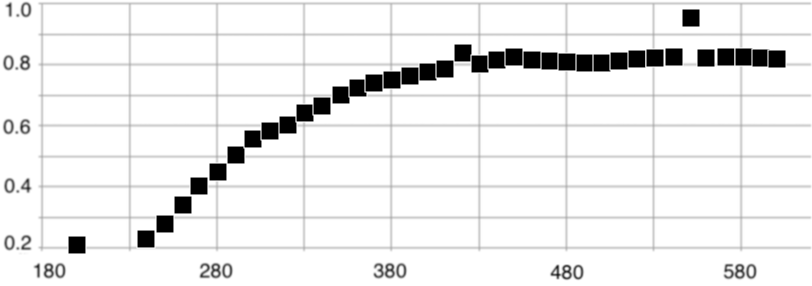
\includegraphics[width=1.0\columnwidth,keepaspectratio]{img/winstoConeSample1Reflectivity.png}
	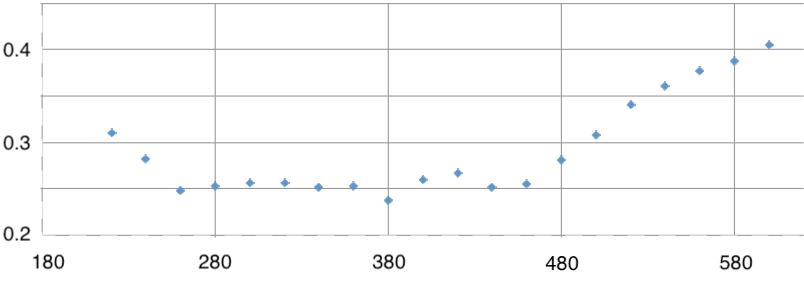
\includegraphics[width=1.0\columnwidth,keepaspectratio]{img/winstoConeSample2Reflectivity.png}
	\caption{Top view of the back-wall of the LTCC. A stainless steel bar encapsulate a sandwich wall of aluminum and foam. On the left and right side
			of the frame a new patch panel allow for 3 hermetical connectors (1 HV, 2 signals) from each PTM. }
	\label{fig:windowDesign}
\end{figure}


